\documentclass{article}

\makeatletter
\renewcommand{\fnum@figure}{Εικόνα \thefigure}
\makeatother

\usepackage[greek, english]{babel}
\usepackage{alphabeta}
\usepackage{atbegshi, picture}

% Set page size and margins
% Replace `letterpaper' with`a4paper' for UK/EU standard size
\usepackage[letterpaper,top=2cm,bottom=2cm,left=3cm,right=3cm,marginparwidth=1.75cm]{geometry}

% Useful packages
\usepackage{amsmath}
\usepackage{graphicx}
\usepackage[colorlinks=true, allcolors=blue]{hyperref}
\usepackage[utf8]{inputenc}
\usepackage{indentfirst}

\addto\captionsenglish{
  \renewcommand{\contentsname}
    {Περιεχόμενα}
}

% \title{Feasibility Study}
% \date{}

\begin{document}
% \maketitle

\begin{titlepage}
   \begin{center}
       \vspace*{1cm}

       \textbf{\huge Project Description}

       \vspace{0.5cm}
        Τεχνολογία Λογισμικού
            
       \vspace{1cm}

       \textbf{Κατερίνα Μητροπούλου\\Μάριος Στεφανίδης}
       
       \begin{figure}[!htb]
        \centering
        
\includegraphics[width=0.5\textwidth]{logo.png}
        \end{figure}
        
        \vspace{0.5cm}
        
        \begin{figure}[!htb]
        \centering
        
\includegraphics[width=0.5\textwidth]{ceid.jpg}
        \end{figure}


       \vfill
            
       Τεχνικό Κείμενο για την Τεχνολογία Λογισμικού\\
            
       \vspace{0.5cm}
            
       CEID, ECE\\
       University of Patras\\
            
   \end{center}
\end{titlepage}



\noindent Η ομάδα μας

\begin{enumerate}
  \item Βεργίνης Δημήτριος, ΑΜ: 10166634 , ECE
  \item Βλαχογιάννης Δημήτριος, ΑΜ: 1067371, CEID
  \item Κούρου Αγγελική, ΑΜ: 1067499 , CEID
  \item Μητροπούλου Αικατερίνα - Quality Manager, ΑΜ: 1067409, CEID
  \item Στεφανίδης Μάριος - Project Manager, ΑΜ:1067458, CEID
\end{enumerate}

{
  \hypersetup{linkcolor=black}
  \tableofcontents
}

\section{Εισαγωγή}
    Στο συγκεκριμένο τεχνικό κείμενο θα δοθεί μια αρχική περιγραφή του έργου που θα υλοποιήσει η ομάδας μας σε φυσική γλώσσα χωρίς τη χρήση τεχνικών όρων και την αναφορά σε τεχνικές και σχεδιαστικές λεπτομέρειες. Επιπλέον, θα παρουσιαστούν κάποια ενδεικτικά mock-up screens ή διαφορετικά κάποιες από τις βασικές οθόνες που θα περιλαμβάνει η εφαρμογή μας, που θα επιδεικνύουν τις βασικές της λειτουργίες. \par
    Η ομάδα μας θα προσπαθήσει να δημιουργήσει ένα λογισμικό βασιζομένη στον ανθρωποκεντρικό σχεδιασμό λαμβάνοντας υπόψιν βασικές μεθόδους αξιολόγησης (expert evaluation), όπως είναι οι 10 κανόνες του Nielsen και Molich (Heuristic Evaluation), 
    το Cognitive Walkthrough κλπ, ώστε η εφαρμογή που θα προκύψει, να είναι εύχρηστη ως προς το χρήστη και το κατά δυνατόν βέλτιστη.
    

\section{Περιγραφή Έργου}

Το σενάριο που έχουμε υπόψιν μας και το οποίο θα μπορούσε να συμβεί στην πραγματική ζωή, είναι το παρακάτω. Ένας πελάτης προσεγγίζει την ομάδα μας προκειμένου να δημιουργήσει ένα εύκολο και εύχρηστο λογισμικό για την διαχείριση ενός ιδιωτικού νοσοκομείου. Στόχος είναι να διευκολυνθεί κυρίως το έργο του ιατροφαρμακευτικού προσωπικού, αφού θα μπορούν να έχουν πρόσβαση σε δεδομένα που αφορούν τους ασθενείς τους ανά πάσα χρονική στιγμή καθώς και να απαλλαχθούν από τις χρονοβόρες γραφειοκρατικές διαδικασίες. Βέβαια, πέρα από την τυπική διαχείριση δεδομένων ενός νοσοκομείου (διαχείριση ασθενών, αποθήκης/φαρμάκων, ραντεβού κοκ), αυτό που θα το ξεχωρίσει από τα ήδη υπάρχοντα λογισμικά που επιτελούν ίδιες ή παρόμοιες ενέργειες, είναι η εισαγωγή κάποιων καινούγιων εννοιών και λειτουργιών, όπως είναι η φωνητική αναζήτηση, προτάσεις για πιθανές εξετάσεις (εξετάσεις αίματος, ακτινογραφίες, αξονικές κοκ) που πρέπει να γίνουν ανάλογα με την αρχική διάγνωση και τα συμπτώματα του ασθενούς και τελική διάγνωση του ασθενούς με τη βοήθεια του ICD-10 Code (Διεθνής Στατιστική Ταξινόμηση Νοσημάτων και Συναφών Προβλημάτων Υγείας), καθώς και η δημιουργία ενός σύγχρονου Graphical User Interface (GUI), το οποίο θα διαφέρει κατά πολύ από αυτά που υπάρχουν ήδη στην αγορά. \par
\textbf{Υποσημείωση:} Λόγω της μεγάλης έκτασης του λογισμικού που επιθυμούμε να υλοποιήσουμε, θα επικεντρωθούμε κυρίως μόνο σε ένα κομμάτι του, το οποίο θα αφορά κυρίως την διαχείριση ασθενών από γιατρούς/νοσηλευτές, την διαθεσιμότητα φαρμάκων και ιατρικών δωματίων (όπως είναι κλίνες, εργαστήρια, χειρουργεία).


\section{Ενδεικτικές Οθόνες}

Σε αυτό το σημείο θα παρουσιαστούν κάποιες ενδεικτικές οθόνες που θα περιλαμβάνει η εφαρμογή μας, το όνομα της οποίας θα είναι \textbf{Medic World}. Σκεφτόμαστε πως κάποιοι από τους χρήστες που θα έχουν πρόσβαση σ' αυτήν, θα είναι οι εξής:

\begin{itemize}
  \item Γιατροί: διαχείριση ασθενών, συμπλήρωση ιστορικού \& συμπτωμάτων, παραγγελία εξετάσεων, έκδοση εξιτηρίου, πρόσβαση στην καρτέλα αποθήκης φαρμάκων
  \item Νοσηλευτές/Νοσηλεύτριες: παρόμοιες λειτουργίες με αυτές του γιατρού με κάποιες προφανείς διαφοροποιήσεις
  \item Admin: διαχειριστής της εφαρμογής, έκδοση κωδικών, διαγραφή χρηστών από το σύστημα, δυνατότητα πρόσβασης στο system log
  \item Φαρμακοποιοί: πρόσβαση στις καρτέλες των ασθενών και στην καρτέλα αποθήκης φαρμάκων
\end{itemize}

Το λογισμικό που αναπτύσσουμε είναι διαθέσιμο σε tablets, τα οποία θα παρέχει το ιδιωτικό νοσοκομείο στους χρήστες, προκειμένου να εκμεταλλευτεί στο έπακρο η δυνατότητα φορητότητας και εξοικονόμησης χρόνου, μιας και η συμπλήρωση στοιχείων ενός ασθενούς μπορεί να γίνει οποιαδήποτε στιγμή, καθώς και σε Η/Υ. Το prototyping tool που χρησιμοποιήθηκε για την δημιουργία των mock-up screens είναι το \textbf{figma}.

\subsection{Οθόνη Εισόδου}

Παρακάτω φαίνεται η οθόνη εισόδου του Medic World. Είναι προφανές πως δεν είναι εφικτή η λειτουργια registration, μιας και οι κωδικοί του κάθε χρήστη θα παραχωρούνται σε αυτόν απευθείας από τη μηχανοργάνωση του νοσοκομείου.

\vspace{0.3cm}

\begin{figure}[!htb]
\centering
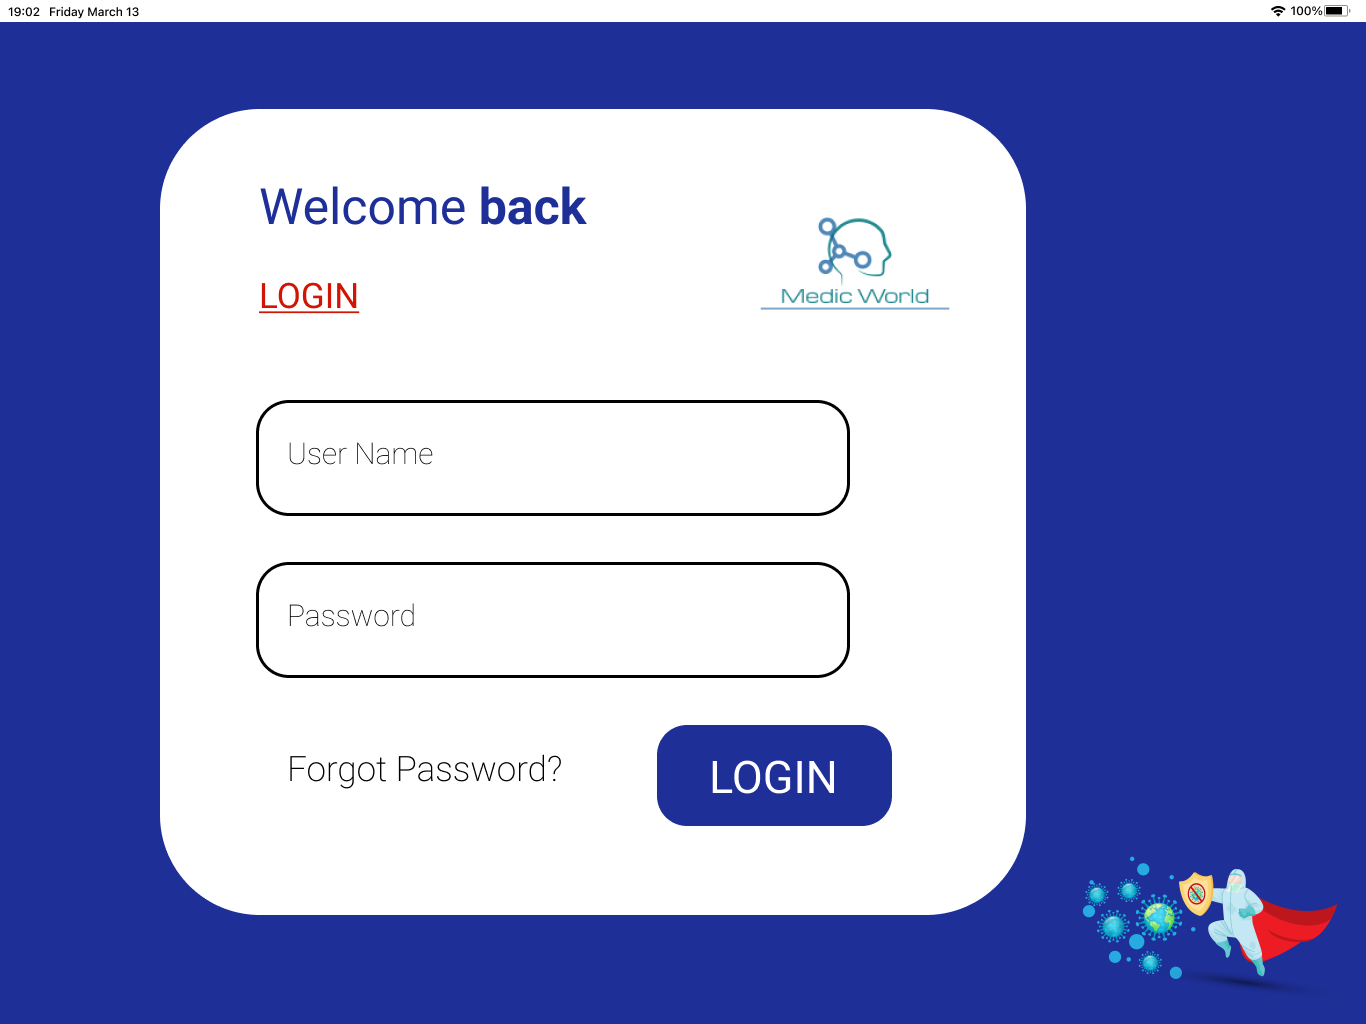
\includegraphics[width=0.5\textwidth]{Log in.png}
\caption{\label{fig:log in page} Οθόνη Εισόδου}
\end{figure}

\subsection{Κεντρική Σελίδα (Γιατρός)}

Σε περίπτωση που συνδεθεί στην εφαρμογή με τους κωδικούς του ένας από του γιατρούς του προσωπικού, θα οδηγηθεί στην αρχική σελίδα που αντιστοιχεί σε αυτήν την επαγγελματική κατηγορία. Κάποιες από τις λειτουργίες που προσφέρει η συγκεκριμένη οθόνη, είναι οι εξής:

\begin{itemize}
  \item Εμφανίζεται το πρόγραμμα που έχει ο γιατρός μέσα στην μέρα
  \item Πρόσφατες ενημερώσεις που αφορούν το νοσκομείο και την διαχείριση των ασθενών, ώστε να παρέχεται πλήρη ενημέρωση
\end{itemize}

\vspace{0.3cm}

\begin{figure}[!htb]
\centering
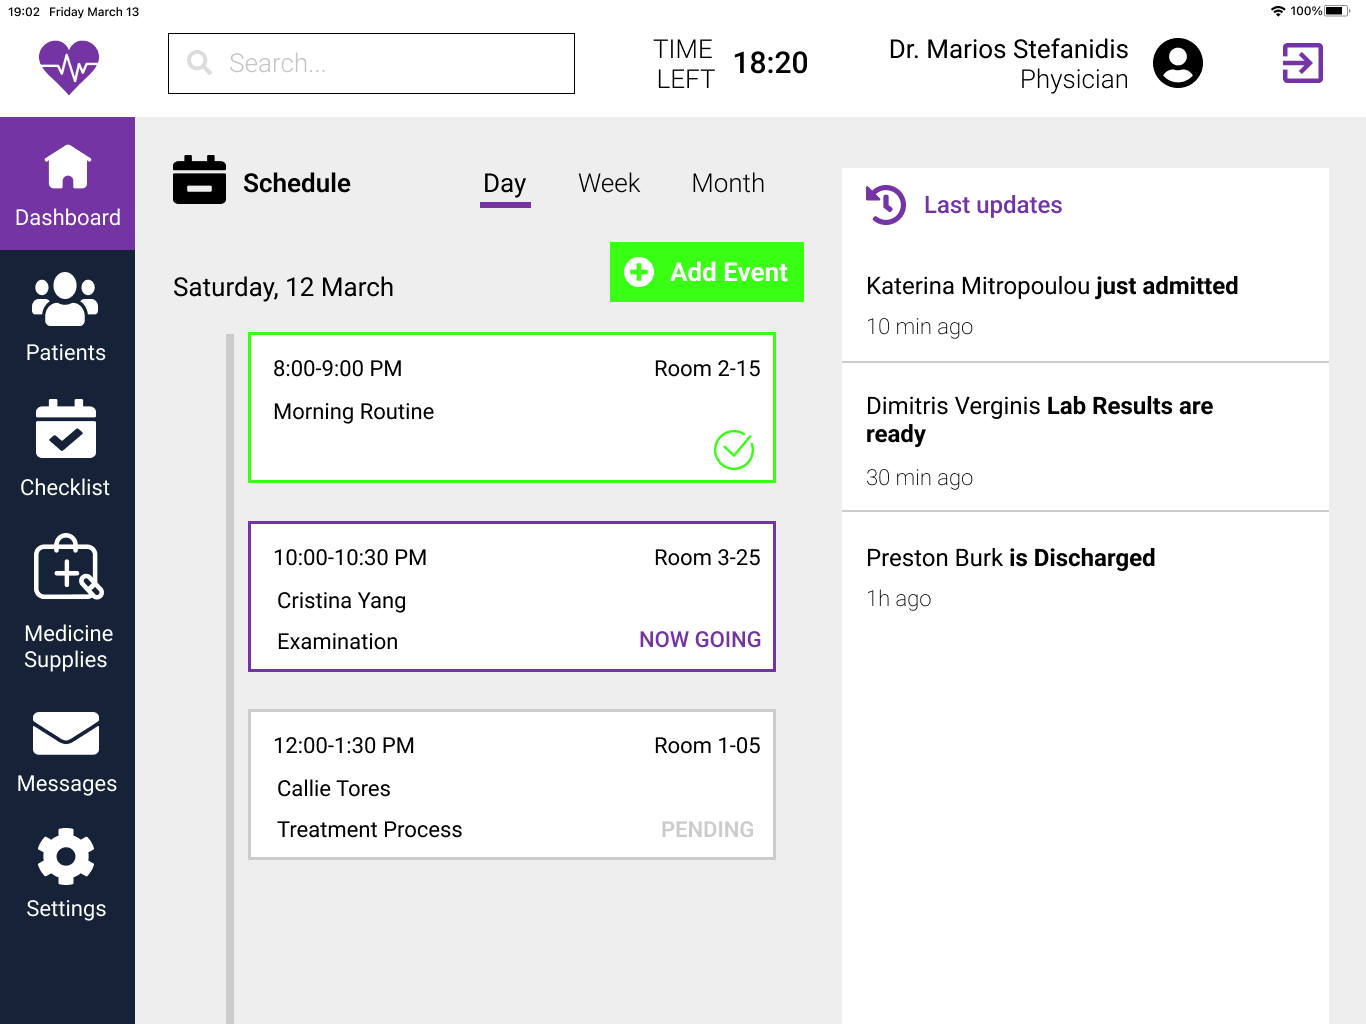
\includegraphics[width=0.5\textwidth]{Main Page (Doctor).png}
\caption{\label{fig:main page} Κεντρική Σελίδα Γιατρού}
\end{figure}


\subsection{Καρτέλες Ασθενών}

Επιλέγοντας το εικονίδιο patients ο χρήστης οδηγείται σε μία λίστα αποτελούμενη από τις καρτέλες των ασθενών. Κάθε καρτέλα περιλαμβάνει βασικές ενδείξεις που χρειάζεται να γνωρίζει ο γιατρός. \par
Η κεντρική ιδεά είναι να εμφανιζόνται οι ζωτικές ενδείξεις των ασθενών που γίνονται monitoring συνεχώς απευθείας στην εφαρμογή. Σε περίπτωση εμφάνισης κάποιας ακραίας τιμής (είτε προς τα κάτω, είτε προς τα πάνω), θα εμφανίζεται αμέσως ειδοποίηση στον γιατρό. 

\vspace{0.3cm}

\begin{figure}[!htb]
\centering
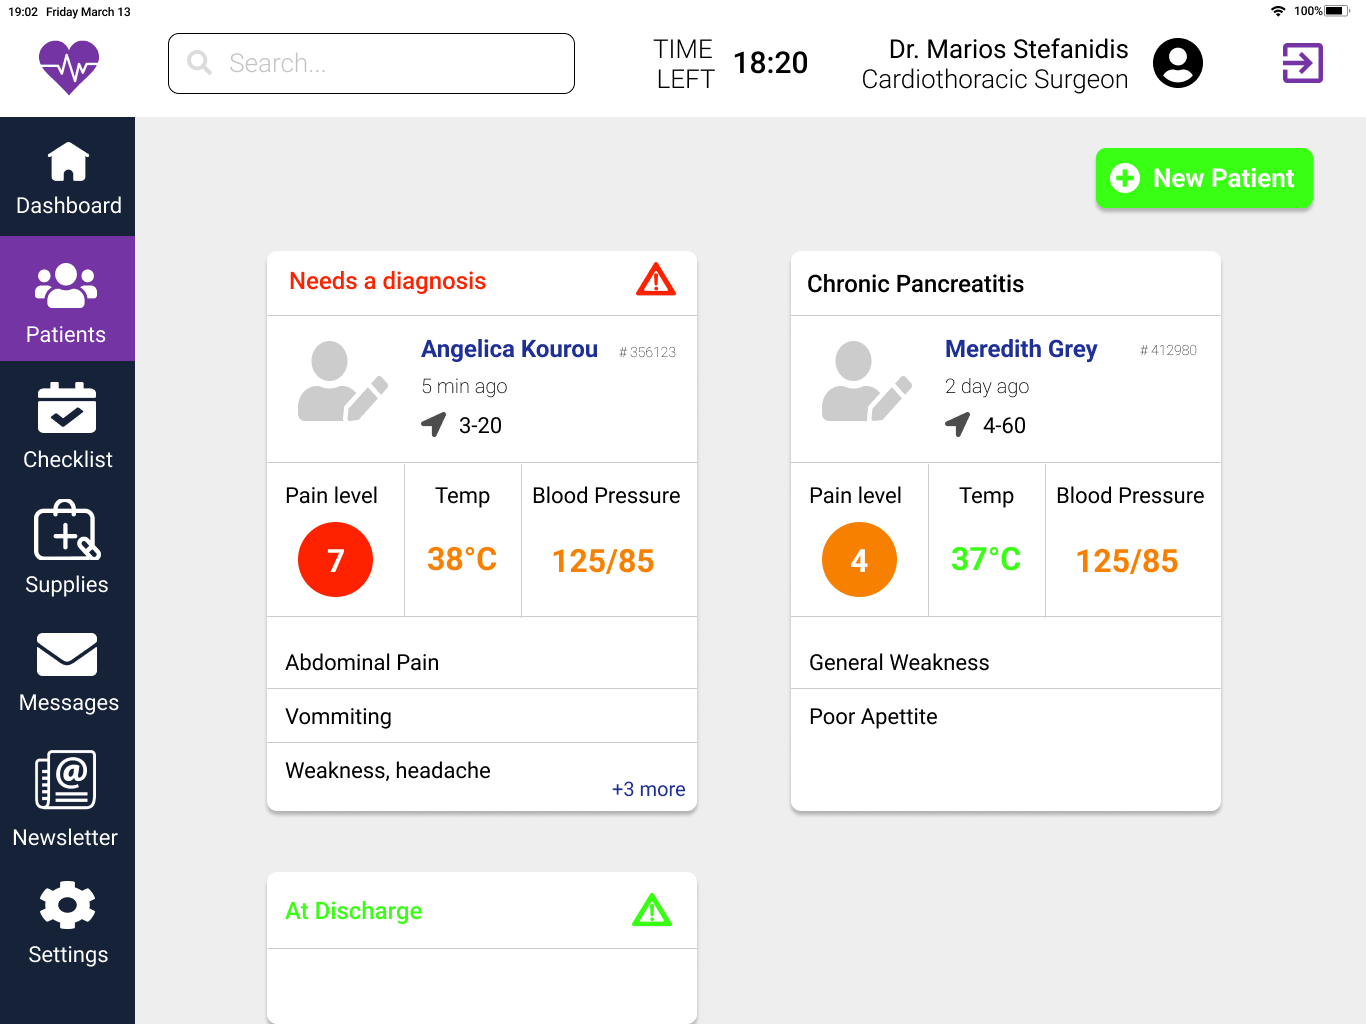
\includegraphics[width=0.5\textwidth]{Patients.png}
\caption{\label{fig:patients cards} Καρτέλες Ασθενών}
\end{figure}

\newpage

\subsection{Προφίλ Ασθενών}

Πατώντας πάνω στο όνομα ενός ασθενούς στην εικόνα 3, εμφανίζεται η εικόνα 4, η οποία περιέχει περισσότερες λεπτομέρειες και σημαντικές πληροφορίες που αφορούν τον συγκεκριμένο ασθενή, όπως είναι η εμφάνιση των εργαστηριακών αποτελεσμάτων (Lab Results), οι οποίες θα εισάγονται στο σύστημα αμέσως μόλις πραγματοποιηθούν και το τελευταίο θα προσπαθεί να εντοπίζει πιθανές "ανωμαλίες" και να τις καταγράφει. \par
Μπορεί ακόμα να πραγματοποιηθεί προσθήκη νέων συμπτωμάτων και ιστορικού με τη χρήση του πληκτρολογίου ή της φωνητικής αναζήτησης. Επίσης, ο γιατρός μπορεί να προσθέσει επιπλέον εξετάσεις (Diagnostic Workup), στις οποίες θα του εμφανίζονται κάποιες προτεινόμενες, σύμφωνα με την αρχική διάγνωση που έχει γίνει και εν τέλει να πραγματοποιεί την τελική διάγνωση.
Θα μπορεί να καταγράφεται με λεπτομερή τρόπο το πλάνο φροντίδας του ασθενούς (care plan), όπως είναι η διατροφή, οι δοσοληψίες φαρμάκων, χειρουργία και να διατηρείται ένα ιστορικό (patient profile) που θα περιλαμβάνει τα δημογραφικά και κλινικά δεδομένα του.

\vspace{0.3cm}

\begin{figure}[!htb]
\centering
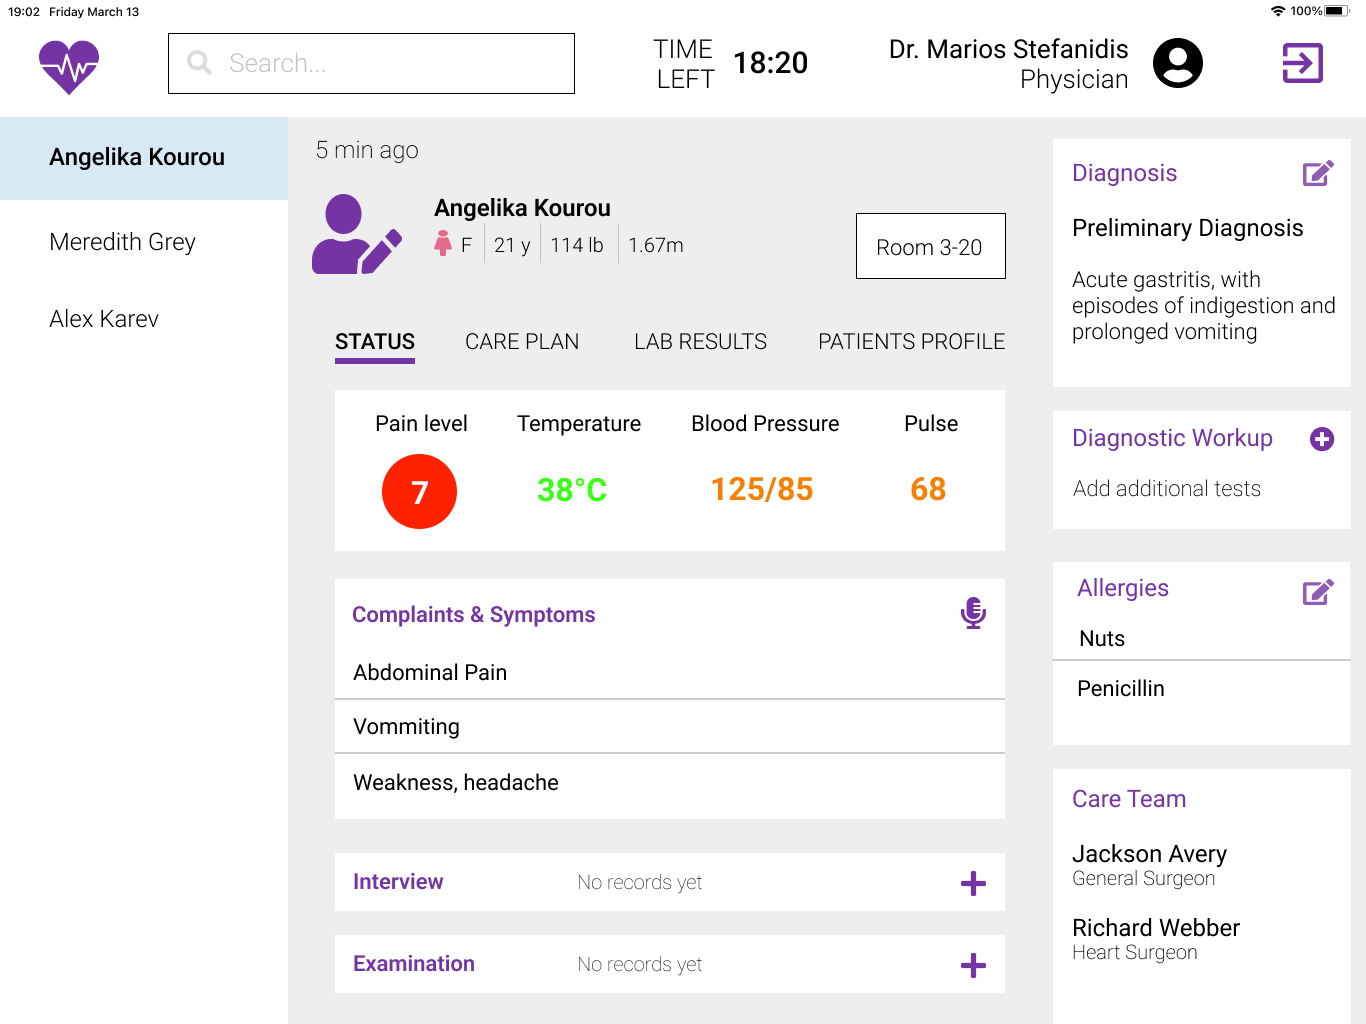
\includegraphics[width=0.5\textwidth]{Patients Cards.png}
\caption{\label{fig:patient profile} Προφίλ Ασθενούς}
\end{figure}


\subsection{Λίστα Ελέγχου}

Μία από τις λειτουργίες που προσφέρει η Medic World είναι ο εκάστοτε χρήστης ανά πάσα στιγμή να είναι σε θέση επιλέγοντας το εικονίδιο checklist να έχει πρόσβαση σε μία αρχική καρτέλα που παρουσιάζει πόσες κλίνες, χειρουργεία και εργαστήρια (πχ ακτινολογικό) είναι διαθέσιμα εκείνη τη στιγμή. Πατώντας στην κάθε κατηγορία θα εμφανίζονται τα εξής:

\begin{itemize}
  \item Laboratories: Τα εργαστήρια που είναι διαθέσιμα για παραγγελία εξετάσεων ή παραδείγματος χάριν οι αξονικοί τομογράφοι που είναι σε λειτουργία
  \item Operating Rooms: Τα χειρουργία που βρίσκονται σε εξέλιξη συνοδευόμενα από κάποιες σημαντικές πληροφορίες, όπως είναι ο γιατρός/οι γιατροί που χειρουργούν, ο ασθενής που χειρουργείται, η επέμβαση που πραγματοποιείται κλπ
  \item Rooms: τα δωμάτια και οι κλίνες που είναι διαθέσιμες
\end{itemize}

\vspace{0.3cm}

\begin{figure}[!htb]
\centering
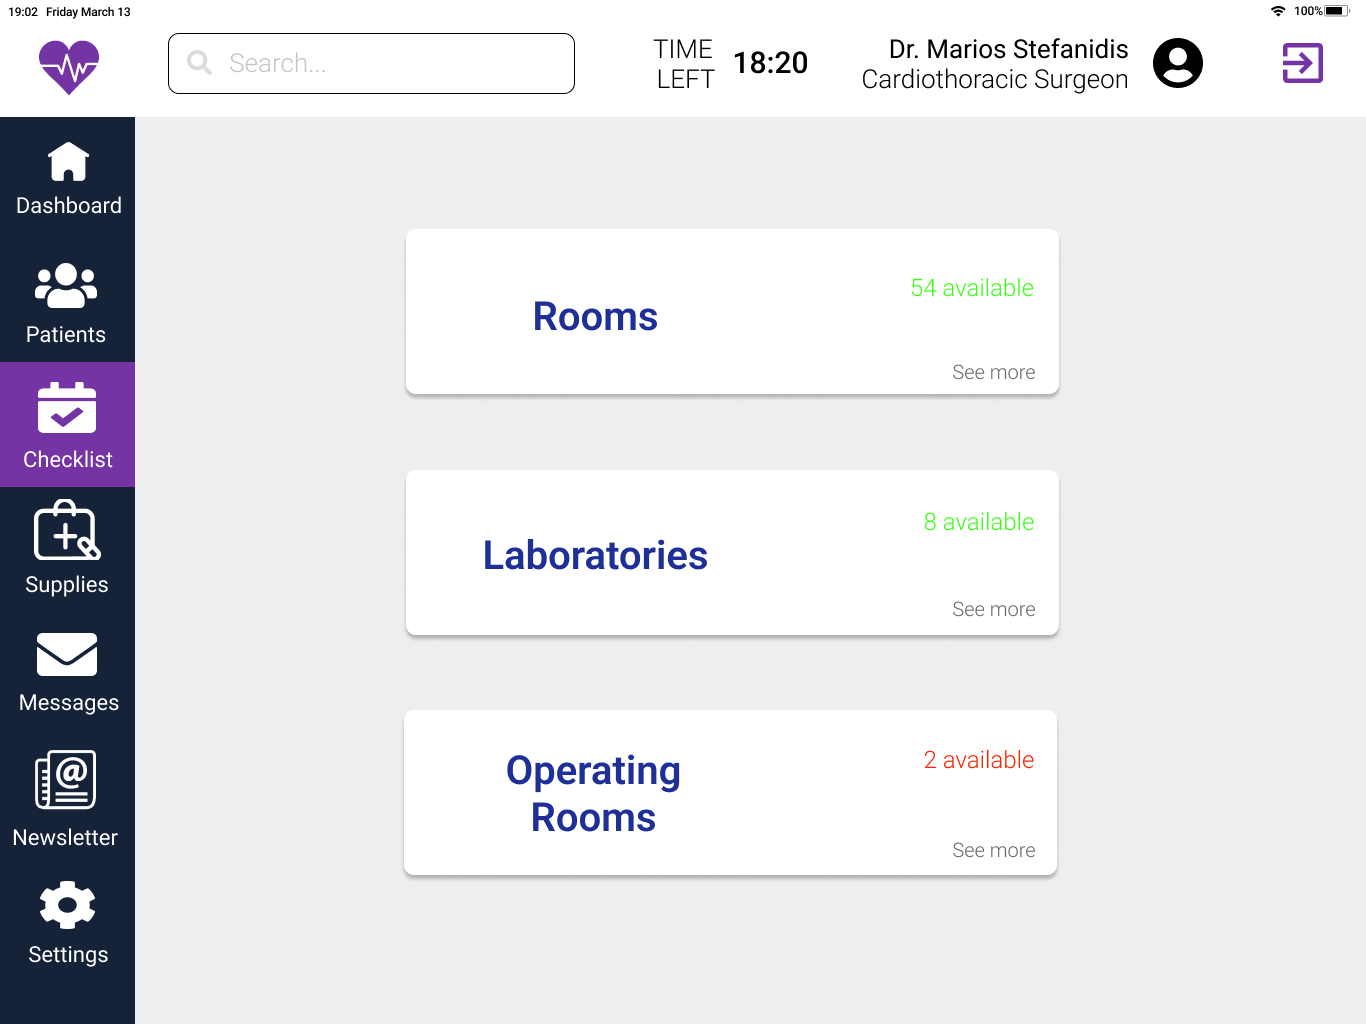
\includegraphics[width=0.5\textwidth]{Checklist.png}
\caption{\label{fig:checklist} Λίστα Ελέγχου}
\end{figure}

\newpage

\subsection{Φαρμακευτικές Προμήθειες}

Τέλος, επιλέγοντας το εικονίδιο που αντιστοιχεί στις φαρμακευτικές προμήθειες ο χρήστης θα οδηγείται σε μία καρτέλα με τα περιεχόμενα της φαρμακαποθήκης. Η λειτουργία αυτή δείχνει στο χρήστη την πληρότητα του νοσοκομείου από το κάθε φάρμακο. Ο υπεύθυνος που διαχειρίζεται την φαρμακαποθήκη, θα μπορεί προφανώς να εκτελεί παραγγελίες των φαρμάκων που βρίσκονται σε έλλειψη, ενώ θα μπορεί να υπάρξει και ένα system log, που θα καταγράφει τα φάρμακα που έχουν χρησιμοποιηθεί και για ποιο λόγο, προκειμένου να αποφευχθούν τυχόν παρανομίες.

\vspace{0.3cm}

\begin{figure}[!htb]
\centering
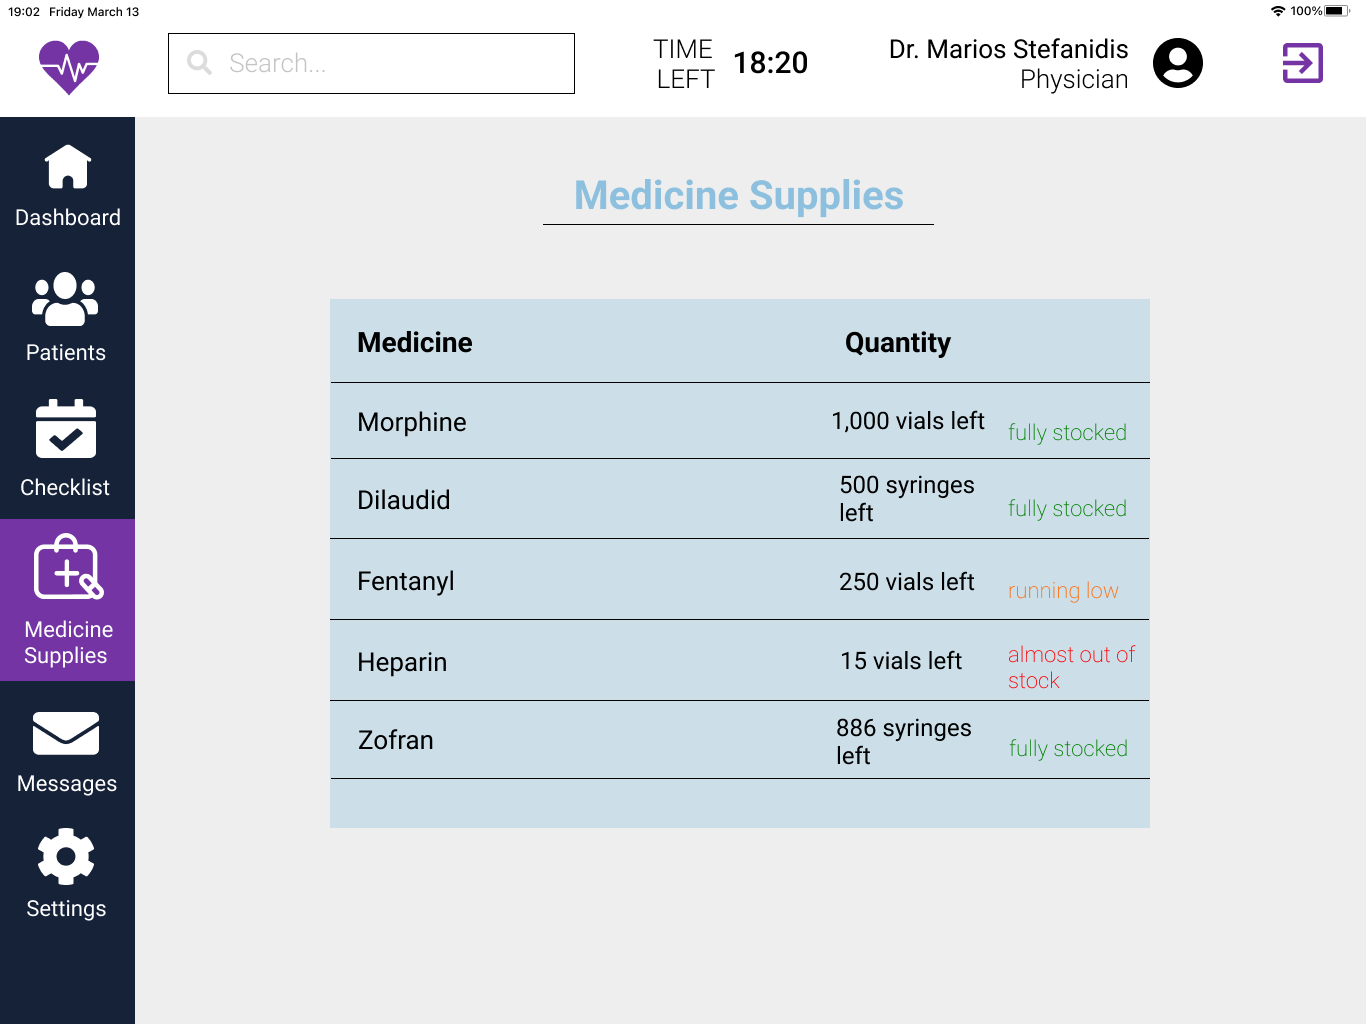
\includegraphics[width=0.5\textwidth]{Pharmaceutical Supplies .png}
\caption{\label{fig:Medical Supplies} Προμήθειες Φαρμάκων}
\end{figure}

\end{document}

